% Ensure you have the following packages in your main.tex:
% \\usepackage{graphicx}
% \\usepackage{booktabs}
% \\usepackage[table]{xcolor}
% \\usepackage{tabularx}
% \\usepackage{float} % For [H] option
% \\usepackage{array} % For advanced table column specifications
% \\usepackage{enumitem} % For custom list labels if needed

% --- Title Page Structure (Adapted from Arabic Example) ---
\begin{titlepage}
    \centering
    {\scshape\Large UNIVERSITY OF ADRAR - AHMED DRAYA \par}
    \vspace{1cm}
    {\scshape\large Faculty of Material Science, Math and Information Technology \par} % Updated
    \vspace{0.5cm}
    {\scshape\large Department of Math and Information Technology \par} % Updated
    \vspace{0.5cm}
    {\scshape\large Specialty: Intelligent Systems \par} % Added
    \vspace{1.5cm}
    {\huge\bfseries DermoSxpert: AI-Powered Digital Healthcare Platform \par}
    \vspace{1cm}
    {\Large\itshape Connecting Patients with Doctors and AI-Driven Skin Cancer Detection\par}
    \vfill
    {\large Supervised by: \par
    Dr. Slimani Ahmed \par}
    % Dr. Supervisor Name 2 (Assistant Supervisor) \par % Corrected if uncommented
    \vspace{2cm}
    {\large Prepared by: \par
    Elmasri Ahmed \par
    Ghanama Ahmed \par}
    \vspace{1cm}
    {\large Date: \par
    \today \par}
    \vspace{1cm}
    % University Logo
    
\includegraphics[width=4cm]{images_pfe/adrar_university_logo.png} % Replace with your university logo if different
    \par
\end{titlepage}

\newpage

% --- Project Technical Sheet (Adapted from Arabic Example) ---
\chapter*{Project Technical Sheet}
\addcontentsline{toc}{chapter}{Project Technical Sheet}

\begin{tabularx}{\linewidth}{@{} l X @{}}
    \toprule
    \textbf{Item} & \textbf{Details} \\\\
    \midrule
    Project Name & DermoSxpert \\\\
    Developer(s) & Elmasri Ahmed, Ghanama Ahmed \\\\
    Legal Status & Startup / Envisioned Company Structure \\\\
    Contact Phone & +213540430098 \\\\
    Contact Email & elmasriahmed.dev@gmail.com \\\\
    Primary Place of Activity & Adrar, Algeria (or as applicable) \\\\
    Incubator/Affiliation & Adrar Incubator\\\\
    Project Domain & Digital Healthcare, Telemedicine, Artificial Intelligence \\\\
    Target Users & Patients in underserved communities, Educational Institutions, General Practitioners \\\\
    Core Technology & Web/Mobile Platform, AI (Deep Learning for image analysis) \\\\
    \bottomrule
\end{tabularx}

\newpage

\chapter{Axis 1: Project Introduction}

\section{Project Idea (Selected Work)}

\textbf{DermoSxpert} is a digital healthcare platform designed to improve access to medical care in underserved communities by connecting users directly with licensed doctors. While it includes an AI-powered tool for early skin cancer detection as a featured capability, the platform’s core mission is broader: to facilitate affordable and accessible healthcare consultations, especially for populations with limited access to medical professionals.

\section{Project Context}

Access to healthcare remains a major issue in many regions, particularly within educational institutions such as high schools, middle schools, religious schools, and Zawiyas. These environments often suffer from poor infrastructure, lack of medical personnel, and weak connections to the national healthcare system. DermoSxpert aims to fill this gap by providing a user-friendly platform that enables remote consultations, increases healthcare awareness, and supports early intervention — all through widely available devices like smartphones and computers.

\section{Team Composition}

DermoSxpert was developed by Elmasri Ahmed and Ghanama Ahmed, a team with expertise in artificial intelligence and full-stack software development, including mobile and web technologies. This compact yet highly capable team enabled rapid development, efficient collaboration, and a clear technical vision aligned with the healthcare needs of underserved populations.

\section{Project Objectives}

The project has several clear objectives:

\begin{itemize}
    \item Improve general access to healthcare in isolated or underserved institutions.
    \item Provide users with the ability to connect with doctors for remote medical advice.
    \item Offer early screening tools, such as AI-based skin cancer detection, to assist in preventive care.
    \item Educate youth and religious communities about common health issues and promote healthy behavior.
    \item Build a sustainable platform that can scale through partnerships with health professionals and institutions.
\end{itemize}

\section{Project Timeline and Development Stages}
The development of DermoSxpert followed an iterative and user-focused process. The key stages are outlined below:

\begin{table}[H]
    \centering
    \caption{Project Development Stages and Timeline}
    \label{tab:project_timeline}
    \rowcolors{2}{LightCyan!20}{white}
    \begin{tabularx}{\linewidth}{@{}lX@{}}
        \toprule
        \rowcolor{Gray}\textbf{Stage No.} & \textbf{Description} \\\\
        \midrule
        1. Needs Assessment & Researching healthcare gaps in educational and religious institutions. Identifying key user requirements and pain points. \\\\
        2. Prototyping & Developing a Minimal Viable Product (MVP) with core features: doctor-patient interface, AI diagnostic tool (skin cancer detection). \\\\
        3. Validation & Collecting feedback from potential users (students, community members) and medical professionals to refine functionality, usability, and design. Iterative improvements based on feedback. \\\\
        4. Business Modeling & Establishing a sustainable monetization strategy. This includes: \\\\
          & \textit{Doctor/Institution Subscriptions:} Healthcare providers pay a fee to be listed and offer remote consultations. \\\\
          & \textit{User Tiers:} Free ad-supported access and a premium ad-free option. \\\\
          & \textit{Referral Commissions:} Receiving a fee when a platform user visits a doctor in person post-consultation. \\\\
        5. Pilot Deployment & Planning limited launches in selected high schools, Zawiyas, and community centers to test real-world performance, gather data, and assess social impact. \\\\
        6. Scaled Launch & Phased rollout to a wider audience based on pilot program success and resource availability. \\\\
        7. Continuous Improvement & Ongoing development, feature enhancement, and AI model updates based on user feedback and technological advancements. \\\\
        \bottomrule
    \end{tabularx}
\end{table}

% Placeholder for a Gantt chart or more detailed visual timeline if available
% \begin{figure}[H]
%     \centering
%     \includegraphics[width=\textwidth]{images_pfe/placeholder_gantt_chart.png} % Replace with your Gantt chart image
%     \caption{Visual Project Timeline (Gantt Chart)}
%     \label{fig:gantt_chart}
% \end{figure}

\chapter{Axis 2: Innovation Aspects}

\subsection{Nature of the Innovation}
DermoSxpert represents both a technological and process innovation in digital healthcare. By integrating a deep learning–based skin diagnostic tool into a user-friendly platform, we enable remote screening that was previously confined to clinical settings. Key points:
\begin{itemize}
  \item \textbf{Technological Innovation:} A convolutional neural network trained on diverse dermatological datasets provides instant risk assessments for skin conditions.
  \item \textbf{Process Innovation:} Streamlined workflows connect users directly with doctors for teleconsultation or in-person follow-up, simplifying access to medical expertise.
  \item \textbf{Radical Impact Potential:} Shifts first-line screening from centralized clinics to any device with a camera, lowering barriers (cost, distance, time) and speeding early detection, which is crucial for conditions like skin cancer.
\end{itemize}

\begin{figure}[H]
    \centering
    % Replace with a diagram illustrating the nature of innovation (e.g., a conceptual model)
   % \includegraphics[width=0.8\textwidth]{images_pfe/placeholder_innovation_diagram.png}
    \caption{Conceptual Diagram: Nature of DermoSxpert's Innovation}
    \label{fig:innovation_nature}
\end{figure}

\subsection{Areas of Innovation}
DermoSxpert innovates across several key areas:
\begin{itemize}
  \item \textbf{Healthcare Access:} Provides remote consultations to underserved populations, significantly reducing travel burdens and wait times, and making specialist advice more readily available.
  \item \textbf{AI-Powered Diagnostics:} Utilizes advanced machine learning to analyze skin images, offering immediate risk assessments for conditions like skin cancer, thereby aiding in early detection and triage.
  \item \textbf{User Engagement and Education:} Combines educational content about skin health with practical diagnostic tools to promote health awareness, preventive care, and informed decision-making among users.
  \item \textbf{Sustainable Business Model:} Implements a multi-faceted business model (subscriptions, referral fees) designed to support ongoing platform development, maintenance, and partnerships with healthcare providers.
  \item \textbf{Community-Centric Focus:} Tailors services to the specific needs and cultural contexts of target communities, including high schools, Zawiyas, and religious institutions, to ensure relevance, trust, and effective adoption.
\end{itemize}

\chapter{Axis 3: Strategic Market Analysis}

\subsection{Target Market}
In its initial phase, the DermoSxpert project targets several key market segments:
\begin{enumerate}
  \item \textbf{Individuals and Consumers:} People interested in their skin health, seeking quick, confidential, and convenient screening solutions, especially those facing difficulty accessing dermatologists due to geographical distance, cost constraints, or long waiting times.
  \item \textbf{General Practitioners and Small Healthcare Institutions:} Clinics and health centers without on-site dermatologists, aiming to streamline initial screening processes, improve diagnostic accuracy for skin conditions, and facilitate timely referrals for their patients.
  \item  \textbf{Educational Institutions:} High schools, middle schools, and religious schools (Zawiyas) that often lack regular on-site access to medical professionals. The platform can serve as a first point of contact for health concerns, particularly skin-related issues.
  \item \textbf{Underserved Communities:} Populations in remote or economically disadvantaged areas with limited healthcare infrastructure, where DermoSxpert can bridge the gap by providing accessible medical consultations and diagnostic support.
\end{enumerate}

\begin{figure}[H]
    \centering
    % Replace with a diagram illustrating the target market segments
   % \includegraphics[width=0.8\textwidth]{images_pfe/placeholder_target_market_diagram.png}
    \caption{DermoSxpert: Target Market Segments}
    \label{fig:target_market}
\end{figure}

\subsection{Market Size and Growth Potential}
The market for digital health solutions, particularly in underserved regions and for AI-driven diagnostics, is rapidly expanding. Key statistics and observations include:
\begin{itemize}
    \item The global telemedicine market size was valued at USD 104.64 billion in 2024 and is projected to grow significantly \cite{fortune2024telemedicine}.
    \item In Algeria, the digital health sector is still in its nascent stages, presenting a substantial opportunity for growth as internet penetration, smartphone usage, and digital literacy increase.
    \item The digital health market in the Middle East and North Africa (MENA) region is expected to witness robust growth, driven by increasing smartphone adoption and government initiatives aimed at improving healthcare access and efficiency.
    \item In neighboring countries like Morocco, the healthcare sector is increasingly adopting digital solutions, with a particular focus on improving access in rural and underserved areas, indicating a regional trend.
    \item A key advantage for DermoSxpert is the relative lack of direct, locally-focused competitors in the Algerian market offering a similar integrated solution (telemedicine + AI skin diagnostics) tailored to local needs, laws, and customs.
\end{itemize}

\subsection{Competitive Landscape}
The competitive landscape for DermoSxpert includes both local and international players in the telemedicine and digital health sectors. However, several factors differentiate DermoSxpert:
\begin{itemize}
  \item \textbf{Local Focus:} Unlike many international platforms, DermoSxpert is tailored to the specific needs, language preferences, and cultural context of Algerian users, ensuring greater relevance, trust, and user adoption.
  \item \textbf{Integrated AI Diagnostics:} The inclusion of an AI-powered skin diagnostic tool as a core feature sets DermoSxpert apart from traditional telemedicine platforms that primarily focus on video consultations without diagnostic assistance.
  \item \textbf{Community Engagement Strategy:} By specifically targeting educational institutions and religious schools (Zawiyas), DermoSxpert aims to build strong community ties and promote health education in a culturally sensitive and impactful manner.
  \item \textbf{Affordable and Accessible Access:} The platform's business model is designed to ensure that users can access essential healthcare services at low or no cost, making it accessible to a wider audience, including those with limited financial means.
  \item \textbf{Partnerships with Local Healthcare Providers:} Collaborating with local doctors, clinics, and healthcare institutions enhances credibility, ensures a continuum of care, and facilitates appropriate follow-up for users.
\end{itemize}

\subsection{Market Entry Strategy}
DermoSxpert's market entry strategy focuses on building strong relationships with key stakeholders and leveraging local networks and community trust:
\begin{itemize}
  \item \textbf{Partnerships with Educational Institutions:} Collaborating with high schools, middle schools, and Zawiyas to integrate DermoSxpert into their health programs, providing students, staff, and their families with easy access to medical consultations and health information.
  \item \textbf{Engagement with Local Healthcare Providers:} Establishing partnerships with local doctors (general practitioners and specialists) and clinics to build a reliable network of healthcare professionals for consultations, referrals, and follow-up care.
  \item \textbf{Community Outreach and Awareness Campaigns:} Conducting awareness campaigns in underserved communities to educate potential users about the platform's benefits, how to access its services, and the importance of early skin health screening.
  \item \textbf{Pilot Programs:} Launching pilot programs in selected institutions and communities to gather real-world feedback, refine the platform based on user experience, and demonstrate its value and impact before broader deployment.
  \item \textbf{Digital Marketing and Social Media:} Utilizing social media platforms and targeted online advertising to reach potential users, particularly younger demographics who are more likely to engage with digital health solutions.
  \item \textbf{User Education and Support:} Providing comprehensive user guides, tutorials, and responsive customer support to ensure a smooth onboarding experience and encourage sustained platform adoption.
\end{itemize}

\chapter{Axis 4: Production and Organization Plan}

\subsection{Production Process (Platform Development \& Operation)}
DermoSxpert’s development and operational model uses a plugin‐based mixture of expert AI models and a robust platform architecture:
\begin{itemize}
  \item \textbf{Expert Model Integration:} Deploy validated AI modules for dermatological analysis (e.g., skin lesion classification). The plugin framework is designed to support future integration of larger multimodal models and search‐enabled AI capabilities.
  \item \textbf{Platform \& API Development:} Build and maintain user-friendly web and mobile clients (for patients and doctors), backend services for managing consultations and data, and integrate with Google/AWS AI APIs as per startup program requirements and for scalability.
  \item \textbf{Rigorous Testing \& Validation:} Conduct comprehensive functional testing, security audits, and clinical validation of AI outputs. Doctor credential verification processes will be implemented in partnership with relevant medical bodies or research labs.
  \item \textbf{CI/CD \& Maintenance:} Implement automated Continuous Integration/Continuous Deployment (CI/CD) pipelines on cloud infrastructure for efficient updates and releases. Continuously monitor platform performance, update AI plugins, and manage user support channels.
\end{itemize}

\subsection{Supply (Key Resources and Suppliers)}
Key resources and suppliers for DermoSxpert include:
\begin{itemize}
  \item \textbf{Cloud AI Services \& Infrastructure:} Leveraging Google Cloud Platform (GCP) and Amazon Web Services (AWS) for scalable compute power, secure storage, and access to advanced AI APIs (in line with startup program benefits).
  \item \textbf{Data Partnerships (Future Goal):} Establishing agreements with hospitals, clinics, and research institutions for access to curated and anonymized dermatological datasets to further train and refine AI models (subject to ethical approvals and data privacy regulations).
  \item \textbf{Software Development Tools:} Utilizing a modern tech stack, including a plugin framework for AI models, and potentially third‐party AI libraries for specialized model management or development.
  \item \textbf{Infrastructure Provisioning \& Monitoring:} Employing automated, cloud‐native provisioning tools (e.g., Terraform, Kubernetes) and robust monitoring systems (e.g., Prometheus, Grafana) for scalability, reliability, and performance tracking.
\end{itemize}

\subsection{Workforce}
The core team initially comprises two software developers with deep AI expertise. Responsibilities and future plans include:
\begin{itemize}
  \item Implement and maintain the expert‐model architecture, platform features, and cloud integrations.
  \item Coordinate with the Adrar incubator and mentors from Google/AWS startup programs for guidance and support.
  \item Manage CI/CD pipelines, provide initial user support, and oversee platform operations.
  \item Outsource specific additional tasks as needed, such as UI/UX design, specialized marketing, and sales representation, particularly during initial growth phases.
  \item \textbf{Future Hiring Plan:} As the platform scales and secures funding, the team plans to expand by hiring additional software developers, data scientists (specializing in medical AI), healthcare liaisons/professionals, marketing specialists, and customer support staff.
\end{itemize}

\subsection{Key Partnerships}
Strategic alliances are crucial for DermoSxpert's success and include:
\begin{itemize}
  \item \textbf{Adrar Incubator:} Access to mentorship, potential seed funding, workspace facilities, and local networking opportunities within the Algerian startup ecosystem.
  \item \textbf{Google/AWS Startup Programs:} Benefits such as cloud credits, technical guidance, and access to AI tools and services, which may require or encourage the use of their respective AI service stacks.
  \item \textbf{Angel Investors \& Venture Capital (Future Goal):} Seeking early‐stage funding from angel investors (e.g., inspired by models like Y Combinator) and later-stage venture capital to fuel growth and expansion.
  \item \textbf{Research Laboratories \& Medical Institutions:} Collaborations for clinical validation of AI tools, model evaluation support, and ensuring medical accuracy and ethical considerations.
  \item \textbf{Healthcare Institutions \& Professionals:} Partnerships for doctor verification, referral commissions, offering teleconsultation services through the platform, and potentially integrating with existing clinic workflows.
  \item \textbf{Educational Institutions \& Community Leaders:} Collaborations to facilitate platform adoption, health awareness campaigns, and pilot programs in target communities.
\end{itemize}

\chapter{Axis 5: Financial Plan}

\subsection{Costs and Expenses (Year 1 Projection)}
\begin{table}[H]
  \centering
  \caption{Projected Costs and Expenses for Year 1}
  \label{tab:costs_expenses}
  \rowcolors{2}{LightCyan!20}{white}
  \begin{tabularx}{\linewidth}{@{} X r @{}}
    \toprule
    \rowcolor{Gray}\textbf{Cost Item} & \textbf{Amount (DZD)} \\
    \midrule
    Research \& Development (AI model integration, platform UI/UX development, backend systems) & 100,000 \\
    Cloud AI Services \& Infrastructure (Google/AWS credits utilization, server costs) & 80,000  \\
    Legal, Regulatory Compliance \& Doctor-verification Setup (consultancy, registration) & 50,000  \\
    Administrative, Marketing \& Launch Activities (office supplies, initial campaigns, promotional materials) & 80,000  \\
    Contingency Reserve (for unforeseen expenses) & 50,000  \\
    \midrule
    \rowcolor{Gray}\textbf{Total Projected Year 1 Expenses} & \textbf{360,000} \\
    \bottomrule
  \end{tabularx}
\end{table}

\subsection{Revenue Streams (Projected)}
\begin{table}[H]
  \centering
  \caption{Projected Revenue Streams and Pricing}
  \label{tab:revenue_streams}
  \rowcolors{2}{LightCyan!20}{white}
  \begin{tabularx}{\linewidth}{@{} X r @{}}
    \toprule
    \rowcolor{Gray}\textbf{Revenue Source} & \textbf{Projected Price/Fee (DZD)} \\
    \midrule
    Doctor Verification \& Listing Fees (per doctor/year, tiered options) & 10,000 \\
    Patient-to-Doctor Referral Fee (per successful in-person referral post-platform use) & 150 \\
    Premium Ad-Free Subscription (per user/year, optional) & 1,000  \\
    Institutional Subscriptions (for schools/organizations, customized packages) & Varies \\
    Data Analytics Services (anonymized, aggregated data for research - future, ethical considerations paramount) & Varies \\
    \bottomrule
  \end{tabularx}
\end{table}

\subsection{Turnover Forecast (3-Year Projection)}
\begin{table}[H]
  \centering
  \caption{Projected Turnover Over Three Years}
  \label{tab:turnover_forecast}
  \rowcolors{2}{LightCyan!20}{white}
  \begin{tabularx}{\linewidth}{@{} X r r r @{}}
    \toprule
    \rowcolor{Gray}\textbf{Description} & \textbf{Year 1 (DZD)} & \textbf{Year 2 (DZD)} & \textbf{Year 3 (DZD)} \\
    \midrule
    \textit{Revenue from Doctors:} & & & \\
    Number of Verified Doctors (cumulative) & 10 & 25 & 50 \\
    Average Verification Fee per Doctor & 10,000 & 10,000 & 12,000 \\
    \quad Total Verification Fees & 100,000 & 250,000 & 600,000 \\
    \midrule
    \textit{Revenue from Users/Patients:} & & & \\
    Number of Ad-Free Subscribers & 50 & 200 & 500 \\
    Subscription Fee per User & 1,000 & 1,000 & 1,200 \\
    \quad Total Subscription Revenue & 50,000 & 200,000 & 600,000 \\
    \midrule
    \textit{Revenue from Referrals:} & & & \\
    Number of Successful Referrals & 100 & 300 & 700 \\
    Referral Fee per Patient & 150 & 150 & 200 \\
    \quad Total Referral Revenue & 15,000 & 45,000 & 140,000 \\
    \midrule
    \rowcolor{Gray}\textbf{Total Projected Turnover} & \textbf{165,000} & \textbf{495,000} & \textbf{1,340,000} \\
    \bottomrule
  \end{tabularx}
  \footnotesize{\textit{Note: These are illustrative projections and subject to market conditions and adoption rates.}}
\end{table}

\subsection{Cash Flow Plan (Simplified Year 1 Overview)}
\begin{table}[H]
  \centering
  \caption{Simplified Year 1 Cash Flow Overview}
  \label{tab:cash_flow_year1}
  \rowcolors{2}{LightCyan!20}{white}
  \begin{tabularx}{\linewidth}{@{} X r @{}}
    \toprule
    \rowcolor{Gray}\textbf{Item} & \textbf{Amount (DZD)} \\
    \midrule
    \textbf{Cash Inflows (Projected)} & \\
    \quad Initial Funding (Seed/Grant) & 360,000 \\\\ % Assuming funding matches expenses for simplicity here
    \quad Revenue (from Turnover Forecast Year 1) & 165,000 \\
    \quad \textit{Total Projected Inflows} & \textit{525,000} \\
    \midrule
    \textbf{Cash Outflows (Projected)} & \\
    \quad Total Projected Year 1 Expenses (from Table \ref{tab:costs_expenses}) & 360,000 \\
    \quad \textit{Total Projected Outflows} & \textit{360,000} \\
    \midrule
    \rowcolor{Gray}\textbf{Net Cash Flow (Year 1)} & \textbf{165,000} \\
    \rowcolor{Gray}\textbf{Ending Cash Balance (Year 1)} & \textbf{165,000} \\
    \bottomrule
  \end{tabularx}
  \footnotesize{\textit{Note: This is a simplified overview. A detailed monthly cash flow would be necessary for operational planning.}}
\end{table}

\subsection{Funding Requirements and Use of Funds}
DermoSxpert seeks initial seed funding of \textbf{360,000 DZD} to cover essential first-year operational expenses and platform development. The allocation of these funds is planned as follows:
\begin{itemize}
  \item \textbf{30\% for Research \& Development (108,000 DZD):} Further development of AI models, platform features, UI/UX enhancements, and backend system robustness.
  \item \textbf{25\% for Cloud AI Services \& Infrastructure (90,000 DZD):} Covering costs associated with cloud computing, data storage, API usage, and ensuring a scalable infrastructure.
  \item \textbf{15\% for Legal, Regulatory \& Setup (54,000 DZD):} Addressing legal consultations, company registration, compliance requirements, and initial doctor verification protocols.
  \item \textbf{20\% for Marketing \& Launch Activities (72,000 DZD):} Initial marketing campaigns, promotional materials, community outreach, and brand building.
  \item \textbf{10\% for Contingency Reserve (36,000 DZD):} To manage unforeseen expenses, market changes, or operational challenges.
\end{itemize}

\chapter{Axis 6: Risk Analysis and Contingency Plan}

\subsection{Risk Identification}
Key risks identified for the DermoSxpert project include:
\begin{itemize}
  \item \textbf{Technical Risks:}
    \begin{itemize}
        \item AI model inaccuracies or biases leading to incorrect diagnostic suggestions.
        \item Software bugs, security vulnerabilities, or platform instability.
        \item Challenges in integrating with existing healthcare IT systems or ensuring data interoperability.
        \item Scalability issues as user base grows.
    \end{itemize}
  \item \textbf{Market Risks:}
    \begin{itemize}
        \item Low adoption rates by patients or healthcare professionals.
        \item Intense competition from existing telemedicine solutions or new entrants.
        \item Changes in healthcare regulations or data privacy laws impacting operations.
        \item Difficulty in achieving projected revenue targets.
    \end{itemize}
  \item \textbf{Operational Risks:}
    \begin{itemize}
        \item Dependence on third-party services (e.g., cloud providers, payment gateways).
        \item Data security breaches or loss of sensitive patient information.
        \item Challenges in scaling customer support and operational processes.
        \item Difficulty in recruiting and retaining skilled technical and medical personnel.
    \end{itemize}
  \item \textbf{Financial Risks:}
    \begin{itemize}
        \item Higher than expected development or operational costs.
        \item Lower than expected revenues or slower monetization.
        \item Difficulty in securing subsequent rounds of funding for growth.
        \item Unfavorable economic conditions impacting user spending or investment.
    \end{itemize}
\end{itemize}

\subsection{Risk Assessment (Illustrative)}
Risks are assessed based on their likelihood and potential impact on the project.
\begin{table}[H]
    \centering
    \caption{Illustrative Risk Assessment Matrix}
    \label{tab:risk_assessment}
    \rowcolors{2}{LightCyan!20}{white}
    \begin{tabularx}{\linewidth}{@{}Xll@{}}
        \toprule
        \rowcolor{Gray}\textbf{Risk Category} & \textbf{Likelihood} & \textbf{Potential Impact} \\\\
        \midrule
        AI Model Inaccuracy & Medium & High \\\\
        Data Security Breach & Low-Medium & Very High \\\\
        Low User Adoption & Medium & High \\\\
        Regulatory Changes & Medium & Medium-High \\\\
        Funding Shortfall & Medium & High \\\\
        Strong Competition & High & Medium-High \\\\
        \bottomrule
    \end{tabularx}
\end{table}

\subsection{Risk Mitigation Strategies}
Proactive strategies will be implemented to mitigate identified risks:
\begin{itemize}
  \item \textbf{Technical Risks Mitigation:}
    \begin{itemize}
        \item Invest in robust AI model training with diverse datasets, rigorous validation, and continuous monitoring for performance and bias.
        \item Implement comprehensive software testing (unit, integration, user acceptance), conduct regular security audits, and follow secure coding practices.
        \item Design a flexible and modular architecture to facilitate easier integration with other systems and ensure scalability from the outset.
        \item Employ redundant systems and backup strategies for critical data and services.
    \end{itemize}
  \item \textbf{Market Risks Mitigation:}
    \begin{itemize}
        \item Conduct thorough market research, user surveys, and pilot programs to understand user needs and refine the value proposition.
        \item Develop a strong brand, unique selling propositions (e.g., local focus, integrated AI), and competitive pricing strategies.
        \item Engage with regulatory bodies proactively to stay informed about upcoming changes and ensure compliance.
        \item Diversify revenue streams and build a strong user community to foster loyalty.
    \end{itemize}
  \item \textbf{Operational Risks Mitigation:}
    \begin{itemize}
        \item Establish strong data security policies, implement end-to-end encryption, and comply with data privacy regulations (e.g., GDPR if applicable, local laws).
        \item Carefully select and manage relationships with third-party service providers; explore multi-cloud or alternative provider options where feasible.
        \item Develop a scalable operational plan, including automated processes and a well-trained customer support team.
        \item Foster a positive work environment and offer competitive compensation to attract and retain talent.
    \end{itemize}
  \item \textbf{Financial Risks Mitigation:}
    \begin{itemize}
        \item Maintain a detailed and realistic financial plan with regular monitoring of key performance indicators (KPIs) and budget variances.
        \item Secure adequate initial funding and maintain a contingency fund to cover unexpected costs or revenue shortfalls.
        \item Develop a clear roadmap for achieving profitability and explore diverse funding sources (grants, angel investors, VCs) for future growth.
        \item Implement cost-control measures and optimize resource allocation.
    \end{itemize}
\end{itemize}

\subsection{Contingency Plan}
In the event of significant unforeseen issues or crises, DermoSxpert will activate its contingency plan, which includes:
\begin{itemize}
  \item \textbf{Financial Contingency:} Utilize the allocated contingency fund to manage immediate financial impacts and stabilize operations.
  \item \textbf{Operational Adjustments:} Temporarily scale back non-essential operations or features to reduce costs and focus resources on critical functions.
  \item \textbf{Stakeholder Communication:} Communicate transparently and promptly with users, investors, partners, and employees about the challenges faced and the steps being taken to address them.
  \item \textbf{Strategic Review:} Conduct a thorough review of the business strategy, market conditions, and operational model to identify necessary pivots or adjustments.
  \item \textbf{Accelerated Funding/Partnership Efforts:} Intensify efforts to secure additional emergency funding, strategic partnerships, or even acquisition if necessary for long-term viability.
\end{itemize}

\chapter{Axis 7: Social Impact and Sustainability}

\subsection{Social Impact Goals}
DermoSxpert is committed to achieving significant positive social impact by:
\begin{itemize}
  \item \textbf{Increasing Access to Healthcare:} Significantly improving access to medical consultations and diagnostic support for underserved populations, particularly those in remote, rural, or economically disadvantaged areas of Algeria.
  \item \textbf{Promoting Early Disease Detection:} Providing essential health screenings (especially for skin conditions like cancer) and educational resources, leading to earlier detection, more timely treatment, and potentially better health outcomes.
  \item \textbf{Reducing Healthcare System Burden:} Easing the load on traditional healthcare facilities by offering an efficient triage system, remote consultations for non-urgent cases, and facilitating appropriate referrals, thereby optimizing resource use.
  \item \textbf{Empowering Individuals:} Equipping individuals with knowledge about their health, user-friendly tools to assess potential health risks (e.g., skin conditions), and direct channels to connect with medical professionals, fostering proactive health management.
  \item \textbf{Strengthening Community Health:} Fostering partnerships with local healthcare providers, educational institutions, and community organizations to build a collaborative health ecosystem and strengthen community health systems.
\end{itemize}

\subsection{Measuring Social Impact}
The social impact of DermoSxpert will be measured through a combination of quantitative and qualitative metrics, including:
\begin{itemize}
  \item \textbf{Access Metrics:}
    \begin{itemize}
        \item Number of registered users from underserved or remote geographical areas.
        \item Number of remote consultations provided, categorized by region and patient demographic.
        \item Reduction in travel time or cost for users accessing medical advice.
    \end{itemize}
  \item \textbf{Health Outcomes (Long-term Tracking):}
    \begin{itemize}
        \item Rates of early skin cancer detection facilitated by the platform (in collaboration with partner doctors).
        \item User-reported improvements in managing skin conditions or accessing timely care.
        \item Feedback from healthcare professionals on the platform's utility in diagnosis and patient management.
    \end{itemize}
  \item \textbf{User Engagement and Satisfaction:}
    \begin{itemize}
        \item Number of active monthly users and user retention rates.
        \item User satisfaction scores (e.g., through surveys, app store reviews).
        \item Feedback on platform usability, information quality, and perceived impact on health decisions.
    \end{itemize}
  \item \textbf{Partnerships and Community Reach:}
    \begin{itemize}
        \item Number and quality of active partnerships with healthcare providers, clinics, and educational institutions.
        \item Number of individuals reached through community health awareness programs linked to the platform.
    \end{itemize}
\end{itemize}

\subsection{Sustainability Strategy}
To ensure long-term sustainability and continued social impact, DermoSxpert will focus on:
\begin{itemize}
  \item \textbf{Scalable and Adaptive Business Model:} Implementing a flexible business model (including diverse revenue streams like subscriptions, referral fees, institutional packages) that can adapt to changing market conditions, user needs, and technological advancements.
  \item \textbf{Continuous Improvement and Innovation:} Committing to ongoing research and development to enhance platform features, improve AI model accuracy, expand service offerings, and incorporate user feedback.
  \item \textbf{Strong Stakeholder Relationships:} Fostering robust and collaborative relationships with healthcare providers, regulatory bodies, community organizations, investors, and users to ensure ongoing support, trust, and collaboration.
  \item \textbf{Diversified Revenue Streams:} Actively pursuing and developing multiple revenue streams to reduce dependence on any single source of income and ensure financial resilience.
  \item \textbf{Alignment of Business and Social Goals:} Maintaining a strong focus on its social mission, ensuring that business objectives and growth strategies consistently align with the overarching goal of improving healthcare access and outcomes for all.
  \item \textbf{Ethical AI and Data Governance:} Upholding the highest standards of ethical AI development, data privacy, and security to maintain user trust and ensure responsible innovation.
\end{itemize}

\appendix
\chapter{Platform UI Mockups (Placeholders)}
\addcontentsline{toc}{chapter}{Appendix: Platform UI Mockups}

This section contains placeholder images for the DermoSxpert platform's user interface. Replace these with actual screenshots or mockups of your application.
\chapter{Platform UI Mockups}
\addcontentsline{toc}{chapter}{Appendix: Platform UI Mockups}

This section contains mockups of the DermoSxpert platform's user interface.

\begin{figure}[H]
    \centering
    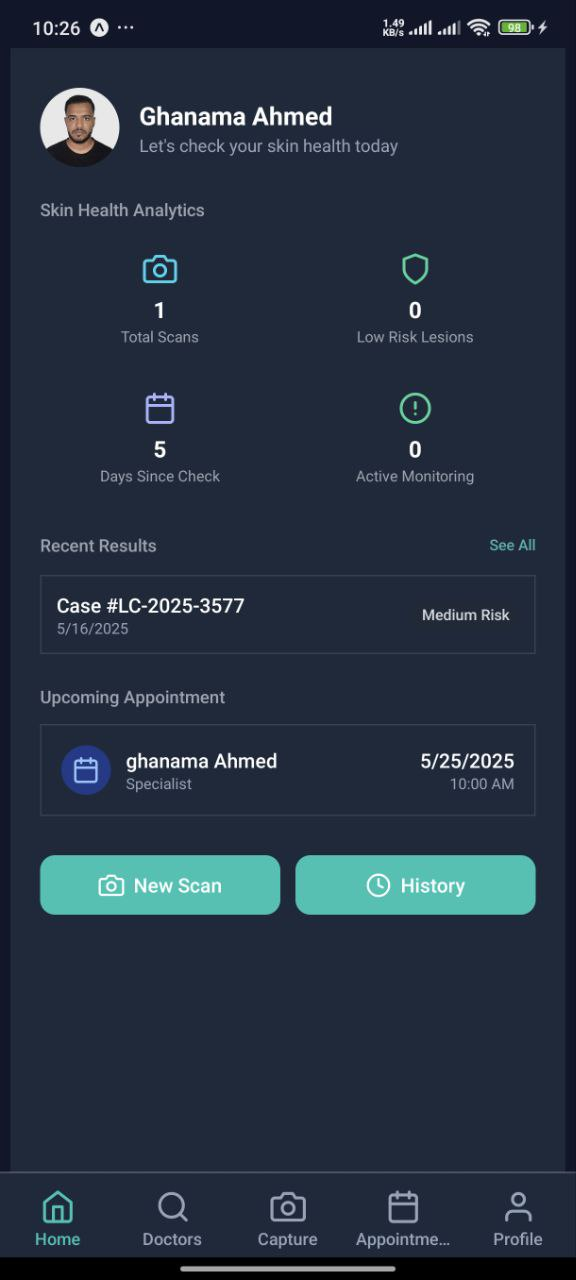
\includegraphics[width=0.5\textwidth]{photo_2_2025-06-01_09-48-58.jpg}
    \caption{DermoSxpert - Main Platform Interface / Homepage}
    \label{fig:ui_main}
\end{figure}




\begin{figure}[H]
    \centering
    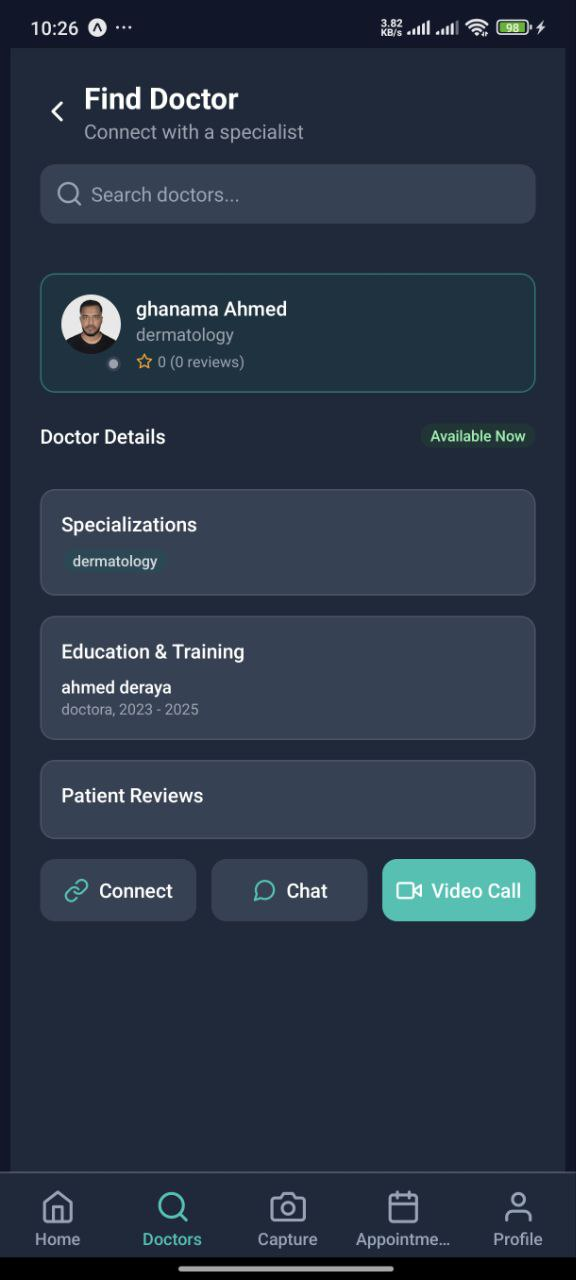
\includegraphics[width=0.5\textwidth]{photo_6_2025-06-01_09-48-58.jpg}
    \caption{DermoSxpert - Service Selection Interface (e.g., Find a Doctor, AI Skin Check)}
    \label{fig:ui_service_selection}
\end{figure}

\begin{figure}[H]
    \centering
    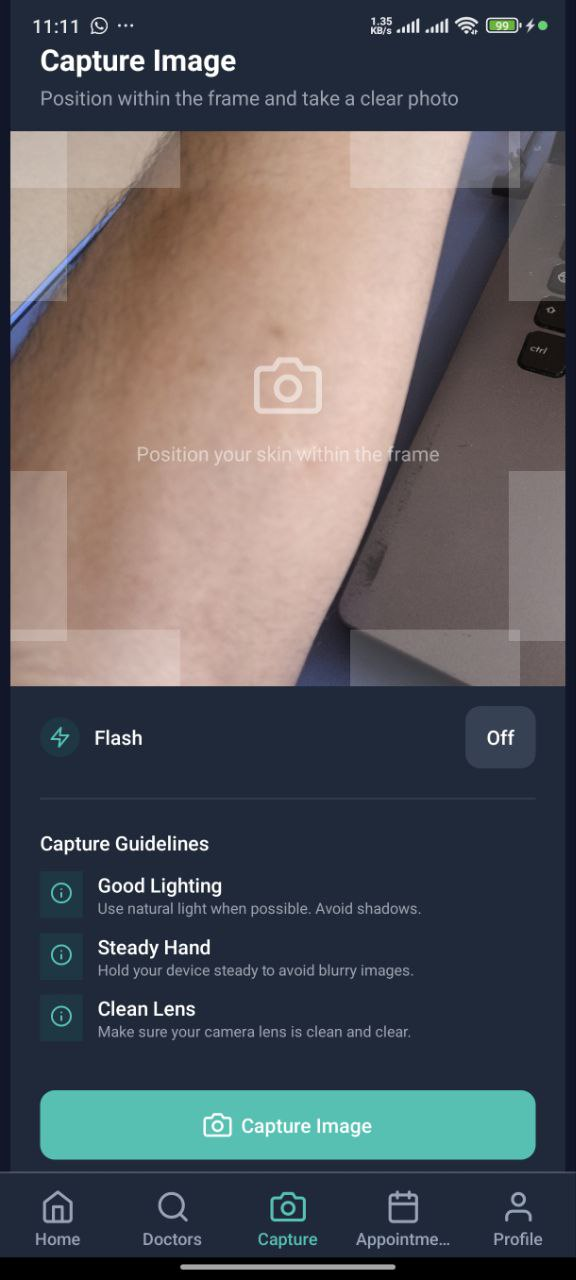
\includegraphics[width=0.5\textwidth]{photo_1_2025-06-01_09-48-58.jpg}
    \caption{DermoSxpert - AI Skin Cancer Detection Tool Interface (Capture Image)}
    \label{fig:ui_ai_tool}
\end{figure}

\begin{figure}[H]
    \centering
    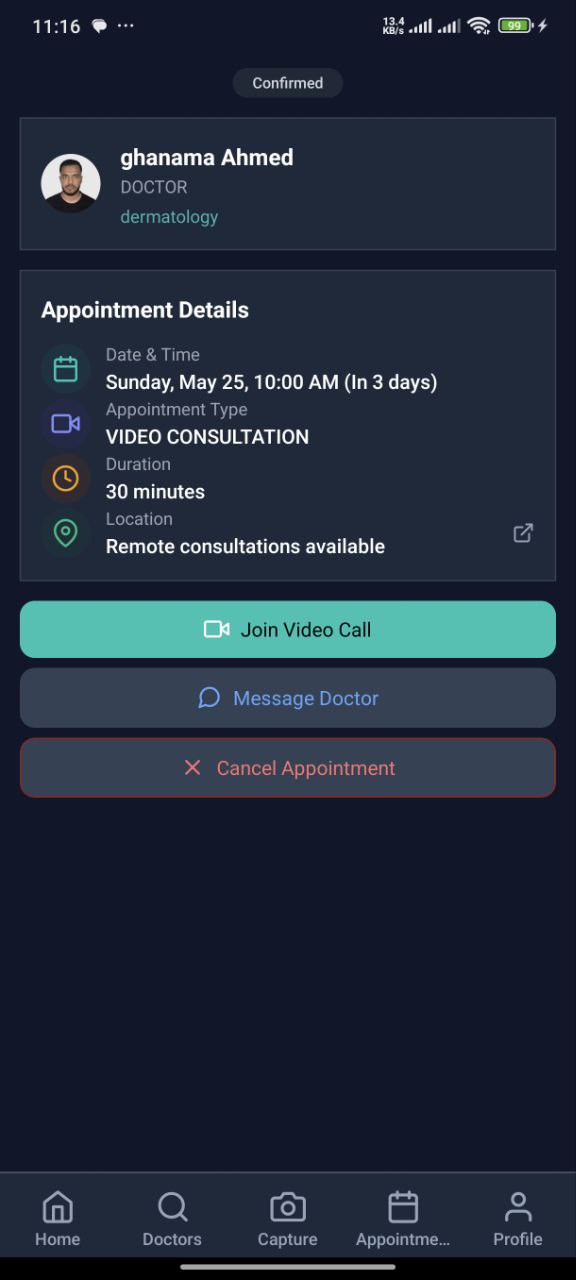
\includegraphics[width=0.5\textwidth]{photo_7_2025-06-01_09-48-58.jpg}
    \caption{DermoSxpert - Doctor's Dashboard / Consultation Interface (Appointment Details)}
    \label{fig:ui_doctor_dashboard}
\end{figure}

\begin{figure}[H]
    \centering
    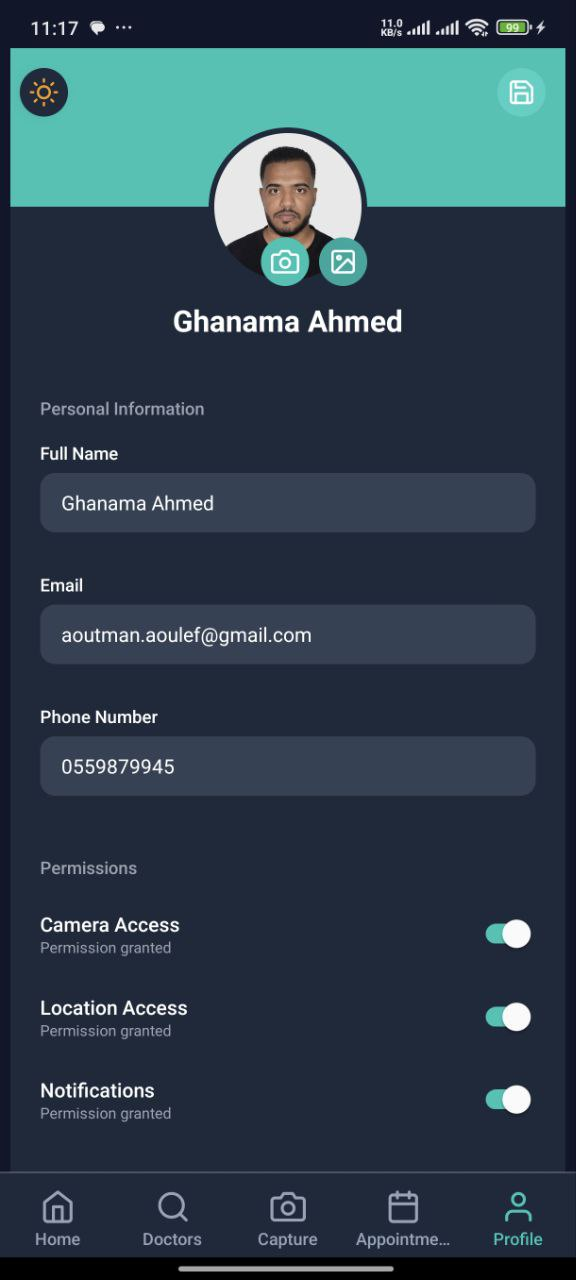
\includegraphics[width=0.5\textwidth]{photo_9_2025-06-01_09-48-58.jpg}
    \caption{DermoSxpert - About the Platform / Information Page (Profile/Personal Information)}
    \label{fig:ui_about}
\end{figure}
% Add more figures as needed for other key UI elements.
